\section{Use Cases}
\subsection{Diagram}
\begin{figure}[H]
   \centering
   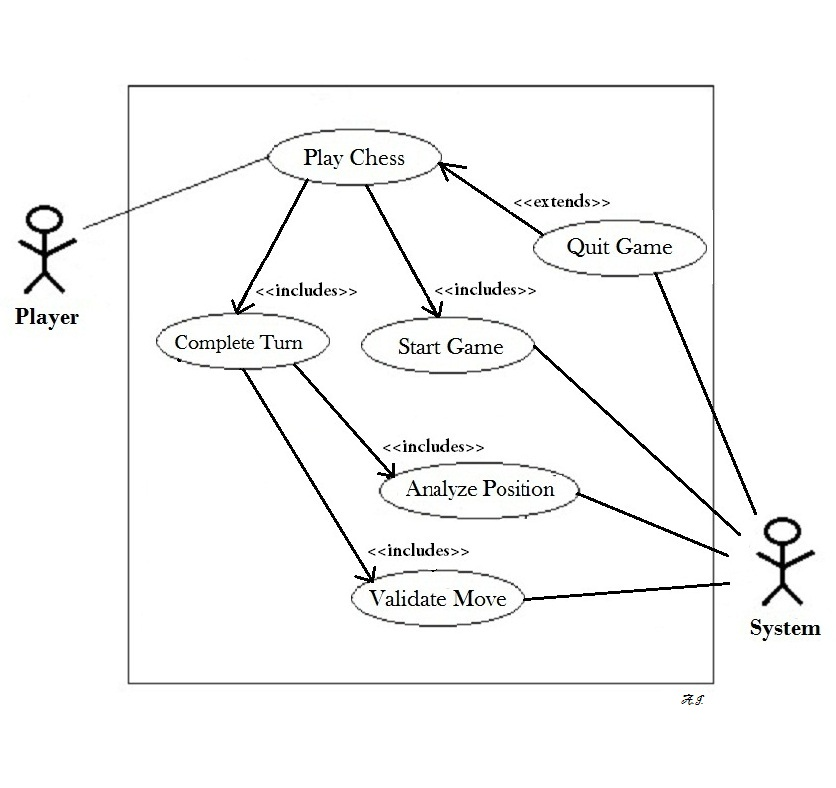
\includegraphics[scale=0.5]{usecase.jpg}
   \caption{Use case diagram for AnonChess}
  \end{figure}
  %\FloatBarrier
\subsection{Flow of Events for the Play Chess Use Case}
\label{playchess}
\subsubsection{Preconditions}
The local player has installed the AnonChess application, and opened the program.
\subsubsection{Main Flow}
This use case begins when the player starts the game (S-10). The player shall engage in a chess match with a remote player (S-20). The use case ends when the system informs the player that the game is over (S-30).
\subsubsection{Sub Flows}
\begin{description}
\item[S-10 Start Game] The player shall start the game per the Start Game use case (\ref{startgame}). 
\item[S-20 Play Game] The player shall alternate completing turns with the remote player, per the Complete Turn use case (\ref{completeturn}). If the player decides to quit the game, the game will not play out to completion (E-10).
\item[S-30 Game Over] The system shall inform the player that the game is over, and the outcome of the game, during the final iteration of the Complete Turn use case (\ref{completeturn}).  
\end{description}
\subsubsection{Alternative Flows}
\begin{description}
\item[E-10 Player Chooses to Quit] extension point- the Quit Game use case  (\ref{quitgame}).
\end{description}

\subsection{Flow of Events for the Start Game Use Case }
\label{startgame}
\subsubsection{Preconditions}
 The program has been initialized.
\subsubsection{Main Flow}
 This use case begins when the player clicks the "Start New Game" button in the AnonChess application, submitting a request to play (S-10). The player shall either start the game with an opponent who is already waiting to play, or have to wait for an opponent to submit a request to play (S-20, S-30). The use case ends when the system initializes a new game (S-40).
\subsubsection{Sub Flows}
\begin{description}
\item[S-10 Submit Request to Play] The player shall click the "Start New Game" button in the AnonChess application, which is the first step to connecting with an opponent (S-20, S-30).
\item[S-20 Connect with Waiting Player] If there is already a person queued to play, the system shall establish a connection(E-10) between the local player and the waiting player.  The system shall display a dialog box stating that the local player has been connected, and start the game (S-40).
\item[S-30 Wait to Connect with Next Available Opponent] If there is no one waiting to play, the system shall display a dialog box stating that the local player is queued to play against the next available opponent who submits a request to play.  If an opponent becomes available within 10 minutes, the system shall start the game (S-40, E-10, E-20).
\item[S-40 Begin New Game] The system shall initialize and begin a chess game between the local player and the remote player.
\end{description}
\subsubsection{Alternative Flows}
\begin{description}
\item[E-10 Connection Cannot be Established] The system shall display a dialog box stating that it could not establish a connection due to technical difficulties, and the player shall be given the chance to submit another request to play (S-10).
\item[E-20 No Opponent Available Within 10 Minutes] The system shall display a dialog box asking the local player if he/she would like to keep waiting.  If the local player does not click “Yes�?, the use case terminates.
\end{description}


\subsection{ Flow of Events for the Quit Game Use Case }
\label{quitgame}
\subsubsection{Preconditions}
  A chess game between the local player and the remote player has been initialized and started per the Start Game use case (\ref{startgame}). 
\subsubsection{Main Flow}
This use case begins when the local player decides to quit, which results in forfeiting the game.  The player shall submit a request to quit (S-10).  The system shall ask the local player to verify his or her wish to quit (S-20). The use case ends when the game is terminated (S-30, E-10).
\subsubsection{Sub Flows}
\begin{description}
\item[S-10 Submit Request to Quit] The local player shall click the "Quit Game" button in the AnonChess application.  The system shall verify the player's resignation (S-20).
\item[S-20 Verify Resignation] he system shall display a dialog box asking the local player to verify his or her decision to quit.  If the local player answers affirmatively (E-10), the system shall terminate the chess game (S-30).
\item[S-30 Terminate Game] The system shall display a message to both the local player and the remote player indicating the remote player has won the game.  The system shall close the remote connection.  The system shall allow the player to create a new game per the Start Game use case (\ref{startgame}). 
\end{description}
\subsubsection{Alternative Flows}
\begin{description}
\item[E-10 Resignation Canceled] The player elects to cancel his or her resignation from the verification dialog box. The program shall close the dialog box and continue per the Complete Turn use case (\ref{completeturn}). 
\end{description}

\subsection{Flow of Events for the Analyze Position Use Case }
\label{analpos}
\subsubsection{Preconditions}
 A player has started a new turn, per the Complete Turn use case (\ref{completeturn})
\subsubsection{Main Flow} 
The use case begins when the system updates the local player's board to reflect the opponent's last move (S-10). Then, the system checks whether or not the local player's King is in a state of Check or Check-Mate (S-20, S-30). The use case ends when the system displays a dialog box stating if special circumstances apply, and returns to the Complete Turn use case (\ref{completeturn}).
\subsubsection{Sub Flows}
\begin{description}
\item[S-10 Update the Board] The system shall update the board with the opponent's last move (E-10), displaying the current positions of the pieces.  If it is the first move of the game, the system shall initialize the board with the pieces in the starting positions.
\item[S-20 Examine Check] The system shall run an algorithm to determine if the local player’s king is under check from any enemy pieces.  If so, the system shall examine whether there is a check-mate (S-30), and if not the system shall proceed to displaying the results of the examination (S-40).
\item[S-30 Examine Check-mate] The system shall run an algorithm to determine if the local player’s king can move to any square that is not under check.  The system shall then display the results of the examination (S-40).
\item[S-40 Display Results] If no special circumstances apply (E-20, E-30) the system shows a dialog box stating that the player can make a move.  The system shall proceed to the Select Piece subflow of the Complete Turn use case (\ref{completeturn}). 
\end{description}
\subsubsection{Alternative Flows}
\begin{description}
\item[E-10 The Received Transmission is Wrong] If the received transmission of the opponent's last move does not match a move in a valid format, the system shall display a dialog box stating that there was an error and allow the opponent to repeat the move per the Complete Turn use case (\ref{completeturn}). 
\item[E-20 Player's King is in Check] The system shall display a dialog box informing the player that he/she must make a move such that the king is no longer in check at the end of the turn, and proceed to the Select Piece subflow of the Complete Turn use case (\ref{completeturn}).
\item[E-30 Check-mate] The system shall display a dialog box that the player has lost the game.  The system shall transmit a message to the opponent, stating the outcome of the game.  The system shall allow the player to create a new game per the Start Game use case  (\ref{completeturn}). 
\end{description}


\subsection{Flow of Events for the Validate Move Use Case}
\label{valmove}
\subsubsection{Preconditions}
The active player has selected a piece to move, and a destination square for the piece per subflows S-30 and S-40 of the Complete Turn use case (\ref{completeturn}).
\subsubsection{Main Flow} 
The use case begins when the system determines what type of piece the player has selected (S-10).  The system verifies that the proposed move is valid according to chess rules that govern movement for the selected piece (S-20, S-30).  The system then updates the board (S-40) and the use case ends when the system transmits the move to the opponent (S-50). 
\subsubsection{Sub Flows}
\begin{description}
\item[S-10 Determine Type of Piece] The system checks whether the player has selected a Pawn, Rook, Bishop, Knight, King, or Queen to move (E-10).
\item[S-20 Validate Standard Move] The system runs an algorithm specific to the type of piece selected to determine if the proposed move is valid.  If the proposed move is not verified as a valid standard move the system checks if it is a valid special move (S-30), otherwise the system updates the board (S-40, E-20)
\item[S-30 Validate Special Move] If the selected piece is a Pawn, the system checks if the proposed move is a valid En Passant move.  If the selected piece is a King, the system checks if the proposed move is a valid Castling move.  If the move is determined to be valid, the system updates the board (S-40, E-20, E-30)
\item[S-40 Update Board]  If the move was determined to be valid then the system shall update the board for the local player so that it stores the move that the player just made.
\item[S-50 Transmit Move] The system shall transmit the details of the move to the opponent in a specified transmission format (E-40), and allow the opponent to make a move per the Complete Turn use case (\ref{completeturn}).
\end{description}
\subsubsection{Alternative Flows}
\begin{description}
\item[E-10 Invalid Piece Selected]  The player selected an area that is not a square containing a playable allied piece.  The player must select another move via the Select Piece subflow of the Complete Turn use case (\ref{completeturn}). 
\item[E-20 Allied King Under Check] if the player's King was under check at the beginning of the turn, the system checks if the King is still in check.  If this is the case, the system displays a dialog box stating that the player cannot finish the turn with the King in check, and the player must select another move via the Select Piece subflow of the Complete Turn use case  (\ref{completeturn}).  If the allied King is no longer in check, the system updates the board (S-40).
\item[E-30 Proposed Move is Invalid] If the proposed move proves not to be valid, the system displays a dialog box stating that the move is invalid and the player must select another move via the Select Piece subflow of the Complete Turn use case   (\ref{completeturn}). 
\item[E-40 Connection Lost] If the system cannot transmit data to the remote player because the connection is no longer active, the game terminates and the system shall allow the player to create a new game per the Start Game use case (\ref{startgame}). 
\end{description}

\subsection{Flow of Events for the Complete Turn Use Case}
\label{completeturn}
\subsubsection{Preconditions} A chess game between the local player and the remote player has been initialized and started per the Start Game use case (\ref{startgame}). It is either the first move of the game, or a transmission of the opponent's last move has just been received per the Complete Turn use case  (\ref{completeturn}). 
\subsubsection{Main Flow}
  This use case begins when it is the local player's turn to move. The system shall update the board and inform the player if there are special circumstances(S-10).  Unless the player is in check-mate, the player shall select an allied piece within the board and a destination square (S-20, S-30).  The use case ends when the move is validated and carried out (S-40).
\subsubsection{Subflows}
\begin{description}
\item[S-10 Check for Special Circumstances] System shall update the board with the opponent's last move, as well as check whether the player's king is in check or check-mate, per the Analyze Position use case (\ref{analpos}). 
\item[S-20 Select Piece] The player shall click one of his or her pieces to select it (E-20). The system shall highlight the selected piece (E-10).
\item[S-30 Select Destination Square]  The player shall click a destination square for the selected piece (E-10).
\item[S-40 Move Piece] The system shall check to see if the requested move follows the rules of chess, and finish the turn per the Validate Move use case (\ref{valmove}) (E-30).
\end{description}
\subsubsection{Alternative Flows}
\begin{description}
\item[E-10 Player Neglects to Select Square] No action is taken, as there is no set time limit for completing moves.
\end{description}
